\chapter{Nuclear Physics and Radioactivity}\index{nuclear physics}\index{radioactivity}

The smoke detector on your ceiling contains a speck of radioactive americium. The banana in
your lunch gives off about 15 tiny bursts of radiation every second. The Sun has been shining
for 4.6 billion years by squeezing hydrogen into helium, and a uranium pellet the size of a
pencil eraser can release as much energy as a ton of coal. All of these happen in the
\emph{nucleus}, the tiny core of the atom, which is 100,000 times smaller than the atom itself
but holds almost all of its mass.

In the Atomic Mass and Chemical Reactions chapter, you met isotopes and the idea of a half-life.
In the Matter and Energy chapter, you used $E = mc^2$ to find the energy released when hydrogen
fuses into helium. This chapter puts those pieces together: what holds a nucleus together, why
some nuclei fall apart, how to calculate how much of a radioactive sample is left, and why both
splitting heavy nuclei and joining light ones release enormous energy.

\section{Inside the Nucleus}\index{nucleus}
A nucleus is made of protons and neutrons, together called \newterm{nucleons}. We write a nucleus
as
$$^{A}_{Z}\text{X}$$
where X is the element's symbol, $Z$ is the \newterm{atomic number} (the number of protons), and $A$
is the \newterm{mass number} (protons plus neutrons). So $^{235}_{\ 92}\text{U}$, uranium-235, has
92 protons and $235 - 92 = 143$ neutrons.

That should surprise you. Protons are positively charged, and the Charge chapter's Coulomb's law
says like charges repel. Two protons 1 femtometer ($10^{-15}$ m) apart, about the width of a nucleus,
push each other apart with a force of
$$F = k\frac{q^2}{r^2} = (8.99 \times 10^9)\frac{(1.60 \times 10^{-19})^2}{(10^{-15})^2} \approx 230 \text{ N}$$
That is about the weight of a large dog, acting on a particle with a mass of only
$1.67 \times 10^{-27}$ kg. Something far stronger must be holding the nucleus together.

That something is the \newterm{strong nuclear force}. It attracts nucleons to each other, protons and
neutrons alike, and at short range it is about 100 times stronger than the electric repulsion. But
it only reaches about the width of a couple of nucleons; beyond that it fades to nothing. Neutrons are
the nucleus's glue: they add strong-force attraction without adding electric repulsion. That is why
heavier nuclei need more and more neutrons to hold together, and why, past lead, no amount of neutrons
is enough to make a nucleus permanently stable.

\section{Radioactive Decay}\index{radioactive decay}
An unstable nucleus eventually changes into a more stable one by emitting radiation. The three most
common kinds are:

\begin{center}
\begin{tabular}{l|p{3.3cm}|p{4.4cm}|p{3.0cm}}
Decay & What comes out & What happens to the nucleus & Stopped by \\
\hline
Alpha ($\alpha$) & a helium-4 nucleus, $^4_2\text{He}$ & $A$ drops by 4, $Z$ drops by 2 & a sheet of paper, or skin \\
Beta ($\beta^-$) & an electron, $^{\ \,0}_{-1}e$ & a neutron becomes a proton: $Z$ rises by 1 & a few mm of aluminum \\
Gamma ($\gamma$) & a high-energy photon & loses energy; $A$ and $Z$ unchanged & thick lead or concrete \\
\end{tabular}
\end{center}

Gamma rays are the highest-energy light in the electromagnetic spectrum from the Electromagnetic
Waves chapter, and each one is a single photon, as in the Photons chapter.

\subsection{Nuclear Equations}\index{nuclear equation}
In every nuclear reaction, the total mass number $A$ and the total charge $Z$ are the same before and
after. That lets you fill in a missing particle by bookkeeping.

\textbf{Example}: Uranium-238 undergoes alpha decay. What does it become?

\textbf{Solution}: $^{238}_{\ 92}\text{U} \to\ ^{A}_{Z}\text{X} +\ ^4_2\text{He}$. Balancing the top
numbers, $238 = A + 4$, so $A = 234$. Balancing the bottom, $92 = Z + 2$, so $Z = 90$. Element 90 is
thorium:
$$^{238}_{\ 92}\text{U} \to\ ^{234}_{\ 90}\text{Th} +\ ^4_2\text{He}$$

\textbf{Example}: Carbon-14 undergoes beta decay:
$$^{14}_{\ 6}\text{C} \to\ ^{14}_{\ 7}\text{N} +\ ^{\ \,0}_{-1}e$$
A neutron turned into a proton, so the carbon became nitrogen, and the mass number stayed 14. (A
nearly massless particle called an antineutrino also escapes, but it does not change the
bookkeeping.)

Your smoke detector uses the alpha decay of americium-241. The alpha particles knock electrons off
air molecules, letting a tiny current flow between two plates. Smoke particles soak up the alpha
particles, the current drops, and the alarm sounds. The alpha particles cannot even get through the
plastic case.

\section{Half-Life}\index{half-life}
You cannot predict when one particular nucleus will decay; it is truly random. But for a large
number of them, the randomness averages out (just as in the Monte Carlo Simulation chapter), and every
radioactive isotope has a \newterm{half-life} $T$: the time for half of any sample to decay.

\begin{center}
\begin{tabular}{l|r}
Isotope & Half-life \\
\hline
Polonium-214 & 164 microseconds \\
Iodine-131 (used to treat thyroid disease) & 8.02 days \\
Cobalt-60 (used in cancer radiation therapy) & 5.27 years \\
Americium-241 (smoke detectors) & 432 years \\
Carbon-14 & 5,730 years \\
Plutonium-239 & 24,100 years \\
Potassium-40 (in bananas, and in you) & 1.25 billion years \\
Uranium-238 & 4.47 billion years \\
\end{tabular}
\end{center}

After one half-life, half the sample remains; after two, a quarter; after three, an eighth. After $t$
years, $\frac{t}{T}$ half-lives have passed, so

\begin{mdframed}[style = important, frametitle = {Radioactive Decay}]
$$N(t) = N_0\left(\frac{1}{2}\right)^{t/T}$$
where $N_0$ is the starting amount and $T$ is the half-life.
\end{mdframed}

This is the exponential decay from the Exponentials and Logarithms chapter. Using
$\left(\frac{1}{2}\right)^{t/T} = e^{-(\ln 2)t/T}$, physicists often write it as $N = N_0e^{-\lambda t}$, with
\newterm{decay constant} $\lambda = \frac{\ln 2}{T}$.

Here is a simulation of 1,000 atoms. In each tenth of a half-life, every surviving atom independently
``flips a weighted coin'' to decide whether it decays:
\begin{minted}{python}
import random

random.seed(8)

atoms = 1000
STEPS_PER_HALF_LIFE = 10
# chance that one atom decays during one step (a tenth of a half-life)
p = 1 - 0.5 ** (1 / STEPS_PER_HALF_LIFE)

for half_life in range(1, 6):
    for _ in range(STEPS_PER_HALF_LIFE):
        # each surviving atom independently decays with probability p
        atoms = sum(1 for _ in range(atoms) if random.random() > p)
    print(f"after {half_life} half-lives: {atoms:4} atoms left "
          f"(formula: {1000 * 0.5 ** half_life:.1f})")
\end{minted}
\begin{verbatim}
after 1 half-lives:  494 atoms left (formula: 500.0)
after 2 half-lives:  249 atoms left (formula: 250.0)
after 3 half-lives:  133 atoms left (formula: 125.0)
after 4 half-lives:   72 atoms left (formula: 62.5)
after 5 half-lives:   34 atoms left (formula: 31.2)
\end{verbatim}

\begin{figure}[H]
\centering
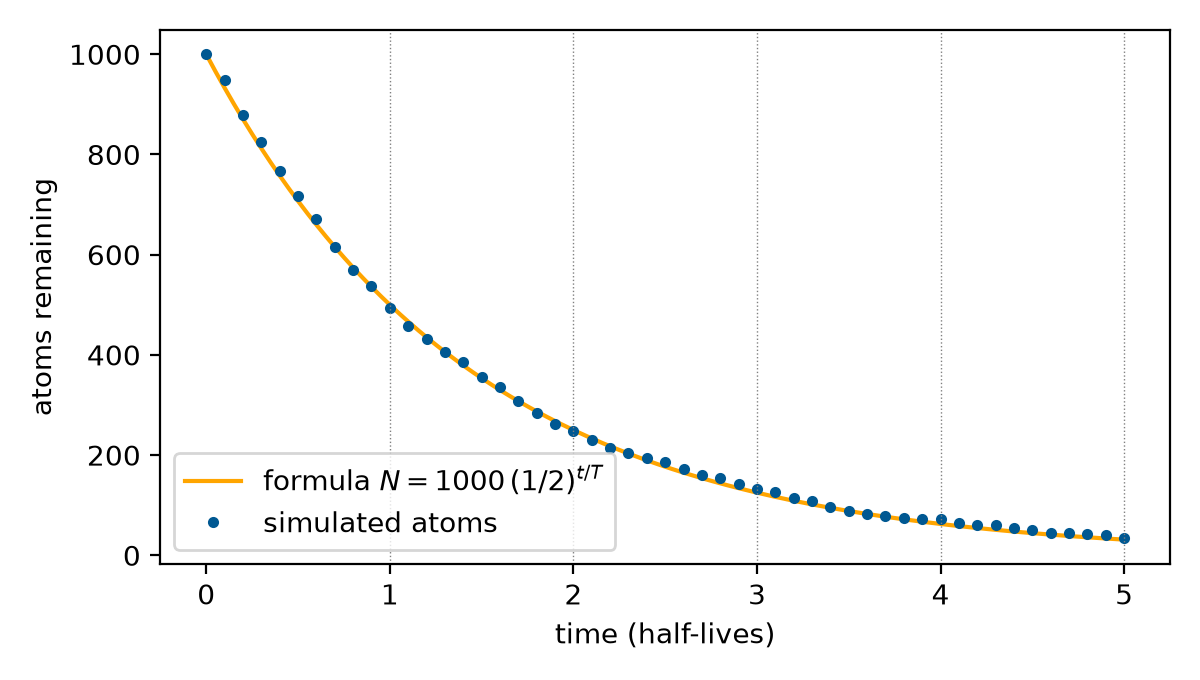
\includegraphics[width=0.75\textwidth]{decay.png}
\caption{Each atom decays at random, yet together they follow the exponential curve.}
\label{fig:decay}
\end{figure}

\subsection{Radiocarbon Dating}\index{carbon-14 dating}
Cosmic rays constantly make carbon-14 in the atmosphere, and living things take it in, so every living
thing has the same small fraction of carbon-14. When an organism dies, it stops taking in carbon, and its
carbon-14 decays. Measure how much is left, and you know how long ago it died.

\textbf{Example}: In 1991, hikers in the Alps found a frozen man, now called \"Otzi. His tissue had about
53\% of the carbon-14 of a living person. How long ago did he die?

\textbf{Solution}: Set $\left(\frac{1}{2}\right)^{t/5730} = 0.53$ and take logarithms of both sides:
$$\frac{t}{5730}\ln\frac{1}{2} = \ln 0.53 \quad\Longrightarrow\quad t = 5730 \cdot \frac{\ln 0.53}{\ln 0.5} \approx 5{,}250 \text{ years}$$
\"Otzi lived more than 5,000 years ago, before the Egyptian pyramids were built.

\section{Mass Defect and Binding Energy}\index{binding energy}\index{mass defect}
Here is a strange fact. A helium-4 nucleus weighs \emph{less} than the two protons and two neutrons it is
made of. Nuclear masses are measured in \newterm{atomic mass units} (u), where
$1\text{ u} = 1.6605 \times 10^{-27}$ kg. Using hydrogen-1 atoms for the protons (so the electrons balance
out):
$$2(1.007825\text{ u}) + 2(1.008665\text{ u}) - 4.002602\text{ u} = 0.030378\text{ u}$$
This missing mass, the \newterm{mass defect}, is the energy that was released when the nucleus formed,
converted by $E = mc^2$. It is also the energy you would have to supply to pull the nucleus apart, so it is
called the \newterm{binding energy}. Nuclear physicists measure it in \newterm{mega-electron-volts} (MeV),
where $1 \text{ MeV} = 1.602 \times 10^{-13}$ J, and $E = mc^2$ works out to $1\text{ u} \to 931.5$ MeV. So
helium-4's binding energy is
$$0.030378 \times 931.5 \approx 28.3 \text{ MeV}, \qquad \text{or about } 7.07 \text{ MeV per nucleon}$$

\begin{figure}[H]
\centering
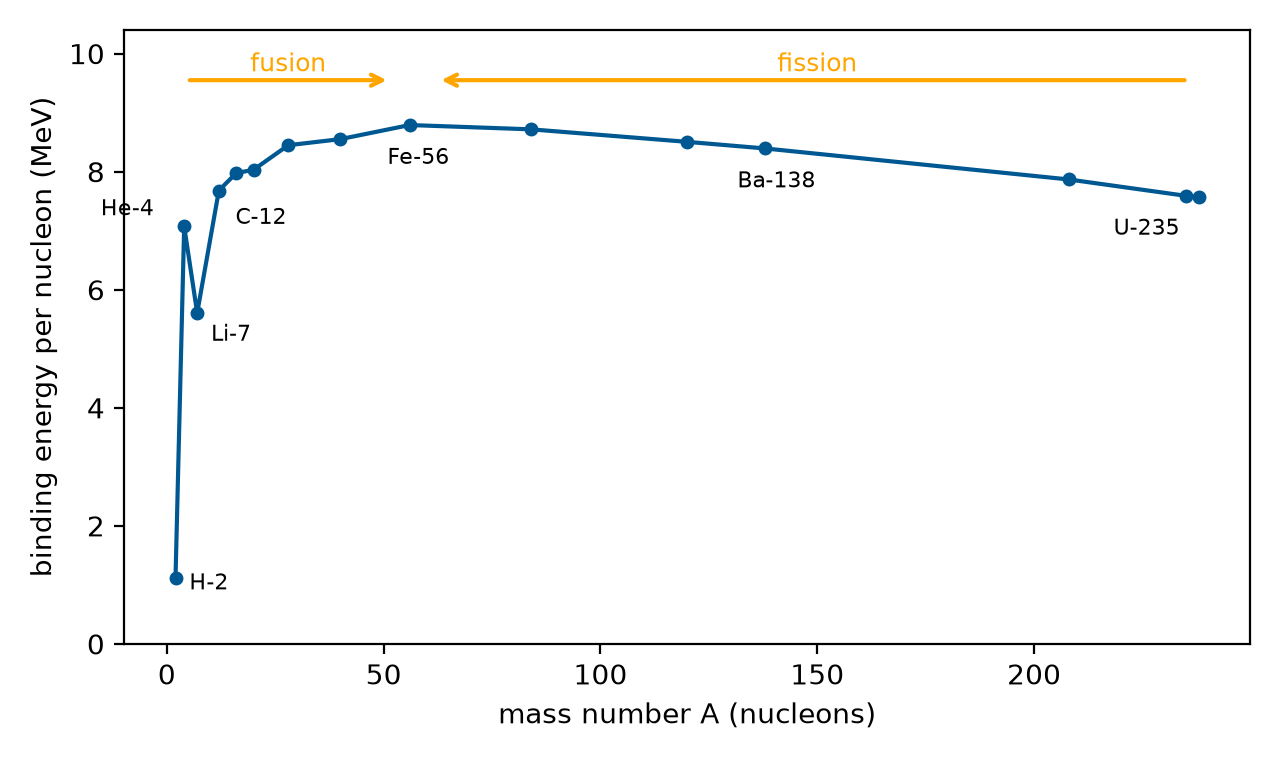
\includegraphics[width=0.85\textwidth]{binding_energy.png}
\caption{Binding energy per nucleon. Iron-56 is near the top: its nucleons are the most tightly bound.
Joining light nuclei (fusion) or splitting heavy ones (fission) moves toward the peak and releases energy.}
\label{fig:binding-energy}
\end{figure}

Figure \ref{fig:binding-energy} is one of the most important graphs in physics. The higher a nucleus
sits on it, the more tightly each nucleon is held, and the more energy was released to make it. The
curve peaks near iron. So there are two ways to release nuclear energy: \emph{join} light nuclei together
(fusion), or \emph{split} heavy nuclei apart (fission). Either way, the products sit higher on the curve
than what you started with, and the difference comes out as energy.

\section{Fission}\index{fission}
When uranium-235 absorbs a slow neutron, it becomes so unstable that it splits in two. One common outcome is
$$^1_0n +\ ^{235}_{\ 92}\text{U} \to\ ^{141}_{\ 56}\text{Ba} +\ ^{92}_{36}\text{Kr} + 3\,^1_0n$$
(Check the bookkeeping: $1 + 235 = 141 + 92 + 3$ and $0 + 92 = 56 + 36 + 0$.) Comparing masses,
$$(235.043930 + 1.008665) - (140.914411 + 91.926156 + 3 \times 1.008665) = 0.186033 \text{ u}$$
so each fission releases about $0.186 \times 931.5 \approx 173$ MeV right away, and more as the fragments
decay. Per kilogram, fissioning uranium-235 releases about $7 \times 10^{13}$ J, roughly 3 million times more
than burning a kilogram of coal.

The key detail is the 3 neutrons. Each can split another uranium nucleus, which releases more neutrons,
and so on: a \newterm{chain reaction}. In a bomb, the chain reaction runs away in a millionth of a second.
In a nuclear power plant, \newterm{control rods} made of neutron-absorbing material soak up just enough
neutrons that, on average, each fission causes exactly one more. The reaction then runs steadily, heating
water to make steam that turns generators, without burning anything or releasing carbon dioxide. The
challenge is the waste: the fission fragments are intensely radioactive, and some stay dangerous for
thousands of years.

\section{Fusion}\index{fusion}
At the other end of the curve, light nuclei release energy by joining. The reaction that engineers are
trying to tame is deuterium (hydrogen-2) plus tritium (hydrogen-3):
$$^2_1\text{H} +\ ^3_1\text{H} \to\ ^4_2\text{He} +\ ^1_0n$$
The mass defect is
$(2.014102 + 3.016049) - (4.002602 + 1.008665) = 0.018884$ u, which is about $17.6$ MeV. Per kilogram of
fuel, that is about 5 times more than fission, and the main product is harmless helium.

So why do we not have fusion power plants? Both nuclei are positively charged, and they must get within the
strong force's tiny range before it can grab them. Pushing them that close against the electric repulsion
takes temperatures above 100 million degrees, hotter than the center of the Sun. The Sun manages at a mere
15 million degrees because its enormous gravity squeezes its core to great density, and because it has
billions of years to wait for the rare collisions that succeed. On Earth, we have to do it in a machine. In
2022, the National Ignition Facility in California crushed a tiny fuel pellet with lasers and, for the
first time, got more fusion energy out than the laser energy that went in. Turning that into a working power
plant is one of the great engineering challenges of your lifetime.

\section{Radiation and You}\index{radiation dose}
Radiation is not something that only exists in power plants. You receive a natural \newterm{background}
dose every day: radon gas seeping from rocks, cosmic rays, and the radioactive potassium and carbon
inside your own body. Doses are measured in \newterm{sieverts} (Sv); natural background gives a typical person about
3 millisieverts per year. A chest X-ray adds about 0.1 mSv. Large doses, many sieverts at once, damage cells
and can be deadly, which is why radiation workers wear badges to track their exposure. The same
cell-killing power, carefully aimed, is used to destroy tumors.

\begin{Exercise}[title={Counting Nucleons}, label=np_count]
How many protons and neutrons are in each nucleus?
\begin{enumerate}
\item $^{56}_{26}\text{Fe}$
\item $^{235}_{\ 92}\text{U}$
\item $^{14}_{\ 6}\text{C}$
\end{enumerate}
\end{Exercise}
\begin{Answer}[ref=np_count]
\begin{enumerate}
\item 26 protons, $56 - 26 = 30$ neutrons.
\item 92 protons, 143 neutrons.
\item 6 protons, 8 neutrons.
\end{enumerate}
\end{Answer}

\begin{Exercise}[title={Complete the Decay}, label=np_decay]
Write the product of each decay.
\begin{enumerate}
\item Radium-226 ($^{226}_{\ 88}\text{Ra}$) undergoes alpha decay.
\item Cobalt-60 ($^{60}_{27}\text{Co}$) undergoes beta decay.
\end{enumerate}
\end{Exercise}
\begin{Answer}[ref=np_decay]
\begin{enumerate}
\item $^{226}_{\ 88}\text{Ra} \to\ ^{222}_{\ 86}\text{Rn} +\ ^4_2\text{He}$. Element 86 is radon, the radioactive gas
that seeps into basements.
\item $^{60}_{27}\text{Co} \to\ ^{60}_{28}\text{Ni} +\ ^{\ \,0}_{-1}e$. Element 28 is nickel.
\end{enumerate}
\end{Answer}

\begin{Exercise}[title={A Medical Isotope}, label=np_iodine]
A hospital receives 100 mg of iodine-131, which has a half-life of 8.02 days.
\begin{enumerate}
\item How much is left after about 24 days (three half-lives)?
\item How much is left after 30 days?
\end{enumerate}
\end{Exercise}
\begin{Answer}[ref=np_iodine]
\begin{enumerate}
\item $100 \times \left(\frac{1}{2}\right)^3 = 12.5$ mg.
\item $100 \times \left(\frac{1}{2}\right)^{30/8.02} \approx 7.5$ mg.
\end{enumerate}
\end{Answer}

\begin{Exercise}[title={How Old Is It?}, label=np_dating]
\begin{enumerate}
\item A bone has 25\% of the carbon-14 of living bone. How old is it?
\item A piece of charcoal has 10\% of the original carbon-14. How old is it?
\end{enumerate}
\end{Exercise}
\begin{Answer}[ref=np_dating]
\begin{enumerate}
\item 25\% is two half-lives: $2 \times 5730 = 11{,}460$ years.
\item $t = 5730 \cdot \frac{\ln 0.1}{\ln 0.5} \approx 19{,}000$ years.
\end{enumerate}
\end{Answer}

\begin{Exercise}[title={Deuterium's Binding Energy}, label=np_deuterium]
A deuterium nucleus is one proton and one neutron. The atomic masses are hydrogen-1, $1.007825$ u;
neutron, $1.008665$ u; and deuterium, $2.014102$ u. Find deuterium's binding energy, and its binding energy
per nucleon. Compare with figure \ref{fig:binding-energy}.
\end{Exercise}
\begin{Answer}[ref=np_deuterium]
The mass defect is $1.007825 + 1.008665 - 2.014102 = 0.002388$ u, so the binding energy is
$0.002388 \times 931.5 \approx 2.22$ MeV, or about $1.11$ MeV per nucleon. That is the lowest point on the curve:
deuterium is barely held together, which is one reason it makes a good fusion fuel.
\end{Answer}

\begin{Exercise}[title={The End of a Star}, label=np_iron]
Large stars fuse lighter elements into heavier ones, all the way up to iron. Use figure
\ref{fig:binding-energy} to explain why fusing iron into anything heavier cannot keep a star shining.
\end{Exercise}
\begin{Answer}[ref=np_iron]
Iron is at the peak of the curve. Fusing iron into heavier nuclei moves \emph{down} the curve, so it
absorbs energy instead of releasing it. When a massive star's core fills with iron, it loses its energy
source and collapses, often triggering a supernova explosion.
\end{Answer}
